\chapter{Rectangular Waveguide (1)}
In the previous chapter, we developed a general approach for analysing wave propagation inside a waveguide. In this chapter, we will consider a waveguide whose cross section is rectangular. This is called a \textbf{Rectangular Waveguide}\index{rectangular waveguide}. This rectangular pipe is assumed to be made of ideal conductor $\sigma = 0$ and the medium filling this waveguide is an ideal dielectric $\sigma = 0$. We are concerned with the propagation and derivation of these parallel waves in a rectangular waveguide referred to as TE and TM modes, using the same general approach in waveguide analysis.

The waveguide in figure~\ref{fig:lec38fig1} shows the x, y and z coordinates in which the electromagnetic wave is propagated. It is propagated along the z direction. $a$ is the width of the guide while the $b$ is the breadth of the guide. In this guide $a \geq b$.

\begin{figure}[h]
\centering
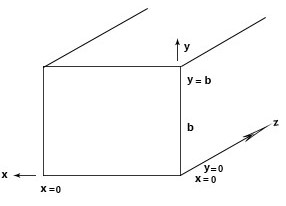
\includegraphics[width=0.7\linewidth]{./graphics/lec38fig1}
\caption{A Rectangular Waveguide}
\label{fig:lec38fig1}
\end{figure}

\section{Transverse Magnetic ($TM$) mode}\index{transverse magnetic mode}
Considering the transverse magnetic (TM mode), $ E_{z} = 0$, $H_{z} = 0 $ longitudinal components. For a transverse field to exist, either $ E_{z} $ or $ H_{z} $ has to be zero. $ H_{z} $ is oriented on the transverse plane and $ E_{z} $ on the longitudinal plane.

Now we first find the solution of the longitudinal component $ E_{z} $ and then find the transverse component $ H_{z} $, and then we apply an initial condition to it. We can use the equations~\ref{eqn:transverseex}-\ref{eqn:transversehy} derived for the TE and TM modes, rewritten as:
\begin{align}
E_x = -\frac{j\omega\mu}{h^2}.\frac{\partial H_z}{\partial y} - \frac{j\beta}{h^2}.\frac{\partial E_z}{\partial x}
\label{eqn:transverseex2}\\
E_y = \frac{j\omega\mu}{h^2}.\frac{\partial H_z}{\partial x} - \frac{j\beta}{h^2}.\frac{\partial E_z}{\partial y}
\label{eqn:transverseey2}\\
H_x = \frac{j\omega\epsilon}{h^2}.\frac{\partial E_z}{\partial y} - \frac{j\beta}{h^2}.\frac{\partial H_z}{\partial x}
\label{eqn:transversehx2}\\
H_y = -\frac{j\omega\epsilon}{h^2}.\frac{\partial E_z}{\partial x} - \frac{j\beta}{h^2}.\frac{\partial H_z}{\partial y}
\label{eqn:transversehy2}
\end{align}
$ \omega $  is the frequency of the wave, $ \mu $   is the permeability of the medium, $ \epsilon $ is the permittivity of the medium filling the waveguide. We expand $ \nabla^{2} $ in the cartesian coordinate system.
\begin{equation}
\frac{\partial ^{2} E_z}{\partial x^2} + \frac{\partial ^2 E_z}{\partial y^2} + \frac{\partial ^2 E_z}{\partial z^2}+ \omega^2\mu\epsilon {E_{z}} = 0
\label{eqn:maxwellele}
\end{equation}

%\begin{figure}
%\centering
%\includegraphics[width=0.7\linewidth]{./graphics/lec38fig2}
%\caption{wave propagation along z}
%\label{fig:lec38fig2}
%\end{figure}
So whatever solution we are going to get for this problem, must have a standing wave kind solution in the x direction with $b\rightarrow \infty$, the same is true if $a\rightarrow \infty$, the standing wave will be in the y direction. Hence, the solution along the x and y directions must be of standing wave type. The solution along the z direction must be of the travelling wave type in the direction of the wave propagation. With this understanding, now we solve the problem. With
\begin{equation}
E_z (x,y,z) = X(x)Y(y)Z(z)
\label{eqn:electricwave}
\end{equation}
Substitute equation~\ref{eqn:electricwave} into equation~\ref{eqn:maxwellele}
\begin{align}
YZ \dv[2]{X}{x} + XZ \dv[2]{Y}{y} + XY \dv[2]{Z}{z}+ \omega^2\mu\epsilon {XYZ} = 0
\end{align}
The partial derivatives have been converted to full ones since $X$, $Y$, and $Z$ are only functions of $x$, $y$, and $z$. Dividing through the expression by $XYZ$ gives
\begin{align}
\frac{1}{X}\dv[2] {X}{x} + \frac{1}{Y}\dv[2]{Y}{y} + \frac{1}{Z} \dv[2]{Z}{z} + \omega^2\mu\epsilon = 0
\label{eqn:diffeqn}
\end{align}
From the equation, $\frac{1}{X}\dv[2] {X}{x}$ is only a function of $x$, $\frac{1}{Y}\dv[2]{Y}{y}$ is only a function of $y$ and $\frac{1}{Z} \dv[2]{Z}{z}$ is only a function of $z$. So this equation that we have written is a \textbf{Point relation}\index{point relation} that should be valid at every point in space. The equation must be satisfied by every point ($x$, $y$, $z$) in the 3D space. That can only happen if $\frac{1}{X}\dv[2] {X}{x}$, $\frac{1}{Y}\dv[2]{Y}{y}$, and $\frac{1}{Z} \dv[2]{Z}{z}$ are constant quantities.

Let,  
\begin{align*}
\frac{1}{X}\dv[2]{X}{x} = -A^2\\
\frac{1}{Y}\dv[2]{Y}{2} = -B^2\\
\frac{1}{Z}\dv[2]{Z}{z} = -\beta^2
\end{align*}
$-A^2$, $-B^2$ and $-\beta^2$ are chosen in such a way that we can always have a standing wave kind of solution in $x$ and $y$ directions while we have a travelling wave solution in the $z$ direction. $\beta$ is the phase constant of the mode of propagation. Thus we have second homogeneous equations as follows:
\begin{align*}
\dv[2]{X}{x} + A^2X = 0\\
\dv[2]{Y}{y} + B^2Y = 0\\
\dv[2]{Z}{z} + \beta^2Z = 0
\end{align*}
Whose solution becomes,   
\begin{align*}
X(x) = C_{1}\cos Ax + C_{2}\sin Ax\\
Y(x) = C_{3}\cos By + C_{4}\sin By\\
Z(x) = C_{5} e^{-j \beta z} + C_{6} e^{+j \beta z}
\end{align*}                                  
The cosine and sine functions show amplitude variation which is a standing wave kind of behaviour. The $C_{5}e^{+j\beta z}$ and $C_{6}e^{-j\beta z}$ are travelling waves in the positive and negative z-direction respectively which indicates the forward and backward travelling waves. So when writing the solution we use our understanding that we have developed from the parallel plane waveguide. That is in the transverse direction, between the two conducting boundaries, we must have a solution that is like a standing wave kind of solution. Along the length of the pipe in which the energy is being propagated, we have a travelling wave kind of solution.

Our solution shows that there are two waves on the structure travelling in the positive and negative z directions. However, if we assume that this waveguide is of infinite $\infty$ distance in the z direction, then there is no reflection. As we have seen from the transmission line, there is no reflection if the transmission line is infinite. So for simplicity of the analysis we assume, there is no wave travelling in the negative z direction and that we have only the forward wave.

Therefore, by substituting the above equations into equation~\ref{eqn:electricwave} we can then write the general equation for the component $E_{z}$. However, for no backward wave, $C_6 = 0$  so that $Z(z) = C_5e^{-\jmath\beta z}$. Thus the general solution for the wave equation $E_z = XYZ$ is
\begin{equation*}
E_{z} = C_{5}(C_{1}cos Ax + C_{2}sin Ax)(C_{3}\cos By + C_{4}sin By) e^{-j\beta z}
\end{equation*}
Now we apply the boundary condition on $E_{z}$ to obtain the constants.  In this case, we are having $E_z$ being tangential to the four walls that make up the waveguide. Hence, we would have four boundary conditions, one for each wall at
\begin{enumerate}[(i)]
\item x = 0
\item x = a 
\item y = 0
\item y = b
\end{enumerate}   
At these four walls, tangential components of electric fields should be zero, i.e. $E_z = 0$ at $x=0$, $x=a$, $y=0$ and $y=b$. At $x=0$,  
\begin{dmath*}
E_{z} = C_{5}(C_1 + 0)(C_3\cos By + C_4\sin By)e^{-\jmath\beta z} = 0
\end{dmath*}
or
\begin{align*}
C_1 C_{5}(C_3\cos By + C_4\sin By)e^{-\jmath\beta z} = 0\\
\longrightarrow C_1 = 0
\end{align*}
$C_1 = 0$ will make $E_z = 0$ for $x=0$ term. At $y=0$,
\begin{dmath*}
E_{z} = C_{5}(C_1 \cos Ax + C_2\sin Ax)(C_3 + 0)e^{-\jmath\beta z} = 0
\end{dmath*}
$C_3 = 0$ will make $E_z = 0$ for $y=0$ so we have reduced $E_z$ to
\begin{dmath*}
E_{z} = C_{5}C_{2}\sin AxC_{4}\sin By e^{-j\beta z} = C_5C_4C_2\sin Ax\sin By e^{-j\beta z}
\end{dmath*}
Let C = $ C_{5}C_{2}C_{4} $
\begin{equation}
E_{z} = C\sin Ax\sin By e^{-j\beta z}
\label{eqn:elesoln}
\end{equation}
Equation~\ref{eqn:elesoln} satisfies the boundary condition $E_z = 0$ at $x=0$ and $y=0$. If $E_z = 0$ at $x=a$ and $y=b$ then
\begin{equation*}
Aa = m\pi,\ A = \frac{m\pi}{a}\footnote{This happens when $\sin Aa = 0$ or $Aa = m\pi$}
\end{equation*}
\begin{equation*}
Bb = n\pi,\ B = \frac{n\pi}{b}\footnote{This happens when $\sin Bb = 0$ or $Bb = n\pi$}
\end{equation*}
$m$ and $n$ are integers. Thus, substituting $A$ and $B$ into equation~\ref{eqn:elesoln}.
\begin{dmath}
E_{z} = C sin\frac{m\pi x}{a} sin\frac{n\pi y}{b} e^{-j\beta z}
\label{eqn:elesoln2}
\end{dmath}
Equation~\ref{eqn:elesoln2} satisfies all four boundary conditions and is the general solution of the wave equation for a rectangular waveguide. $C$ represent the amplitude of the electric field and has nothing to do with the boundary conditions. Since boundary conditions are satisfied irrespective of the power level or the amplitude of the field, $C$ will remain as it is. When we talk about the power inside the mode, only then will the constant $C$ be evaluated. The two quantities $m$ and $n$ now represent the order of the mode, by the same token as what we have done for the parallel plane waveguide when we had a mode and put an index. Now we put two indices for $m$ and $n$. So a transverse magnitude mode can now be designated by $TM_{mn}$ and $m$ is the index around in the broader dimension, $a$, and the $n$ is the index around the shorter dimension, $b$. So the first index tells the field variations along the broader dimension of the waveguide, which is the x direction and the second index tells the field variations along the shorter dimension of the waveguide. 

If $m=1$, from 0 to a, we have one half-cycle variation. If $m=2$, we have two half-cycle variations and so on. Hence this behaviour is essentially identical to what we have seen for the parallel plane waveguide in that the order or index which we have in the mode represents the number of half-cycles in the transverse direction. $m$ in this case are two transverse directions, one in x and another in y. So along x and y, $m$ and $n$ represent the number of half-cycle variations for the field. 

In equation~\ref{eqn:elesoln2}, suppose $a$ or $b$ tends to infinity, it becomes a parallel plane waveguide and then the equation which has for $E_z$ by satisfying either $a=\infty$ or $b=\infty$. Now that we have the constants $m$ and $n$, there are a few things which should be noted. First, $m = 0$ and $n=0 \Rightarrow E_z = 0$. This means that $TM_{00}$ cannot get excited inside a rectangular waveguide.

For parallel plane waveguide, $TM_0$ mode which was the same as $TEM$ mode was possible and it was the \textbf{lowest order} mode. However, for this mode with $m=n=0$, $E_z$ goes to zero in the rectangular waveguide. So $TM_{00}$ does not exist. Also, we note that when any of the indexes go to zero, then $E_z$ goes to zero. $H_z$ is always zero for transverse magnetic mode, so with $E_z$ and $H_z$ going to zero, all fields (all depend on $E_z$ and $H_z$) will identically go to zero. 

\section{Dispersion Relation}
From equation~\ref{eqn:diffeqn} if we substitute the constants, then
\begin{dmath*}
-A^2 - B^2 - \beta + \omega^2\mu\epsilon = 0
\end{dmath*}
But $A=\dfrac{m\pi}{a}$ and $B=\dfrac{n\pi}{b}$ so,
\begin{align}
-\left(\frac{m\pi}{a}\right) - \left(\frac{n\pi}{b}\right) - \beta^{2} + {\omega^2\mu\epsilon} = 0
\label{eqn:hrec}
\end{align}
\begin{equation}
\beta = \sqrt{{\omega^2\mu\epsilon} - \frac{m\pi}{a} - \frac{n\pi}{a}}
\label{eqn:dispersionrelatn}
\end{equation}
This equation is similar to that of the parallel plane waveguide $\bar{\beta} = \sqrt{\omega^2\mu\epsilon - \left(\dfrac{m\pi}{a}\right)}$ where $a=d$ the height of the waveguide. Hence equation~\ref{eqn:dispersionrelatn} tells how the velocity varies as a function of frequency.
\begin{dmath*}
v_p = \frac{\omega}{\beta} = \frac{\omega}{\sqrt{{\omega^2\mu\epsilon} - \frac{m\pi}{a} - \frac{n\pi}{a}}}
\end{dmath*}
Equation~\ref{eqn:dispersionrelatn} is called the \textbf{dispersion relation}\index{dispersion relation} for a transverse magnetic mode on a rectangular waveguide. So this is the dispersion relation for $TM_{mn}$ mode when either $m$ or $n$ is not zero. 

Comparing eqaution~\ref{eqn:hrec} with equation~\ref{eqn:h}.
\begin{dmath*}
h^{2} =  \frac{m\pi}{a} + \frac{n\pi}{b}
\end{dmath*} 
So when $m$ and $n$ are both non-zero, then $h^2$ is not zero. When $h^2$ is not zero, the field will have transverse fields represented in terms of longitudinal components $E_z$ and $H_z$. From the equations for the transverse fields in equations~\ref{eqn:transverseex2}-\ref{eqn:transversehy2} rewritten here,
\begin{align*}
E_x = -\frac{j\omega\mu}{h^2}.\frac{\partial H_z}{\partial y} - \frac{j\beta}{h^2}.\frac{\partial E_z}{\partial x}\\
E_y = \frac{j\omega\mu}{h^2}.\frac{\partial H_z}{\partial x} - \frac{j\beta}{h^2}.\frac{\partial E_z}{\partial y}\\
H_x = \frac{j\omega\epsilon}{h^2}.\frac{\partial E_z}{\partial y} - \frac{j\beta}{h^2}.\frac{\partial H_z}{\partial x}\\
H_y = -\frac{j\omega\epsilon}{h^2}.\frac{\partial E_z}{\partial x} - \frac{j\beta}{h^2}.\frac{\partial H_z}{\partial y}
\end{align*}
If both $E_z$ and $H_z$ are zero, and $h$ is non zero all transverse fields go to zero and so no transverse field exists. $h$ is non zero means $m$ and $n$ are non zero. Hence we can see that for a transverse magnetic mode when either $m$ or $n$ is zero, then $E_z=0$ and $h\neq 0$, the transverse fields will go to zero and the mode will not exist.

So we have important conclusions to derive as follows:
\begin{enumerate}[(i)]
\item $TM_{00}$ does not exist
\item $TM_{m0}$ and $TM_{0n}$ also do not exist
\item $TM_{11}$ is the lowest order of TM mode which can exist on the waveguide.
\end{enumerate}
So we conclude that if the $TM$ mode must be excited in the rectangular waveguide, the field must vary in the x and y direction along the rectangular waveguide. With $m=0$, no variation of fields along the x direction and no variation along the y axis when $n=0$. If $E_z \neq 0$, at $m=0$, $E_z=0$ at $x=0$ and at $x=a$. If there should be no variation, then $E_z$ has to be identically zero everywhere. This is true along the $y$ direction also. This makes sense physically as $E_z$ cannot exist without a variation in the x and y direction. We have also seen from the solution in the cartesian coordinates that the variation is always sinusoidal going in terms of the number of half cycles ($m$ and $n$) in the x or y direction. So the fields in the transverse direction always vary sinusoidally in the cartesian coordinate system. It must vary else the field cannot exist inside. These are the important conclusions which we can draw for the transverse magnetic mode.

Once we get $E_z$, we can substitute into equations for the transverse fields, equations~\ref{eqn:transverseex2}-\ref{eqn:transversehy2}, with $H_{z} = 0$ for $TM$.
\begin{dmath*}
E_x = -\frac{j \beta}{h^2}\cdot\pdv{E_{z}}{x} = -\frac{j \beta}{h^{2}}\cdot\left(\frac{m\pi}{a}\right) C\cos \left(\frac{m\pi x}{a}\right)\sin \left(\frac{n\pi y}{b}\right)e^{-j \beta z}
\end{dmath*}
\begin{dmath*}
E_y = -\frac{j \beta}{h^2}\cdot \pdv{E_z}{y} = -\frac{j \beta}{h^{2}}\left(\frac{n\pi}{b}\right) C \sin\left(\frac{m\pi x}{a}\right)\cos \left(\frac{n\pi y}{b}\right)e^{-j \beta z}
\end{dmath*}
\begin{dmath*}
H_x = \frac{j \omega\epsilon}{h^2}\cdot\pdv{E_z}{y} = \frac{j \omega\epsilon}{h^{2}}\cdot\left(\frac{n\pi}{a}\right) C \sin \left(\frac{m\pi x}{a}\right)\cos \left(\frac{n\pi y}{b}\right)e^{-j \beta z}
\end{dmath*}
\begin{dmath*}
H_y =-\frac{j \omega\epsilon}{h^2}\pdv{E_z}{x} = -\frac{j \omega\epsilon}{h^{2}}\left(\frac{m\pi}{b}\right) C \cos \left(\frac{m\pi x}{a}\right)\sin \left(\frac{n\pi y}{b}\right)e^{-j \beta z}
\end{dmath*}

Now we get the amplitude field for the $TM$ mode in a rectangular waveguide. With the understanding that the lowest order mode in the structure will be $TM_{11}$ mode. With $E_z = C\sin\left(\dfrac{m\pi x}{a}\right)\sin\left(\dfrac{n\pi y}{b}\right)e^{-\jmath\beta z}$, we see that $E_z = 0$ cross-section of the waveguide as shown in figure~\ref{fig:lec38fig3}, the variation of the field in the half-cycles is shown based on the different values of m and n.
\begin{figure}[h]
\centering
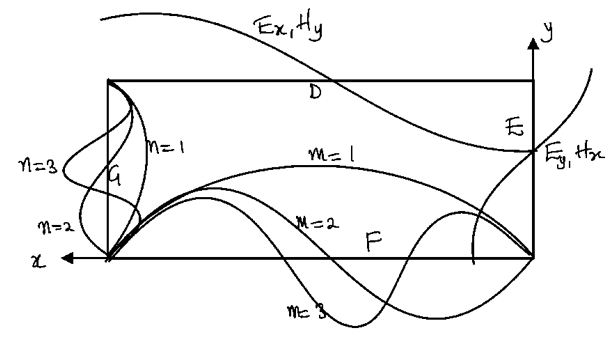
\includegraphics[width=0.7\linewidth]{./graphics/lec38fig3}
\caption{TM mode patterns}
\label{fig:lec38fig3}
\end{figure}
Comparing $E_x$ which we derived with 
\begin{dmath*}
E_x = K \times \cos\left(\frac{m\pi x}{a}\right)\sin\left(\frac{n\pi y}{b}\right)
\end{dmath*}
For $m=1$, $K\cos\left(\dfrac{\pi x}{a}\right)\sin\left(\dfrac{n\pi y}{b}\right)$. $x=0$ gives maximum, $x=a$ gives a negative minimum. So the field of $E_x$ with $m=1$ still has the half-cycle variation like $E_z$, but the maximum and minimum points differ from that of $E_z$. $E_y$ field has cosine variation along y with $m=1$ we have just half-cycle going in the form shown in figure~\ref{fig:lec38fig3}.

So components $E_x$ and $E_y$ will be staggered in space with respect to the $E_z$ component (longitudinal component). Once we have this understanding, we see that $E_x$ and $H_y$ have the same behaviour comparing their expressions. What we observe from here and from the rigorous analysis is that the cross-section of the waveguide shown in figure~\ref{fig:lec38fig3} as D, E, F, and G which are the sides of the waveguide are
\begin{enumerate}[(i)]
\item $H_y$ is tangential to sides E and G of the waveguide
\item $H_y$ is maximum and side E pointing in the position y direction reduces as you move away towards the left side of E. It goes to zero at $x=\dfrac{a}{2}$, changes direction and starts increasing in the opposite direction till it is maximum again at $x=a$ ( in the opposite direction to that at $x=0$). 
\end{enumerate}
This variation of $H_y$ is sinusoidal to make a certain number of half-cycles depending on the order of mode. Similarly 
\begin{enumerate}[(i)]
\item $H_x$ is tangential to sides D and F of the waveguide
\item $H_x$ at D is maximum and points in the position x direction; it reduces as you move upward to 0 at $y=\dfrac{b}{2}$ the middle point. Beyond this point, it changes direction till it gets to another maximum at F which is opposite it its original maximum at D. 
\end{enumerate}
The number of half-cycles depends on order n. Hence, this explanation is based on $n=1$. We looked at only the variations of $E_x$ along y, to have $E_x = K\sin\left(\dfrac{n\pi y}{b}\right)$. $E_x$  is also tangential to sides D and F of the waveguide. With $n=1$, $E_x = K\sin\left(\dfrac{\pi y}{b}\right)$. So at $H_x = $ maximum, say $y=0$, $E_x = 0$ because of sinusoidal variations. $H_x$ was a cosine variation at $Y=\dfrac{b}{2}$, $E_X = $ maximum, whereas $H_x = 0$ at that point.

Whatever magnetic field on the tangential surface is balanced by the surface current so that the boundary conditions of the tangential component of the magnetic field can hold. So the magnetic field is maximum on the conducting boundary and having understood that the solution gives a sinusoidal variation in the transverse direction. The same inference can be made for the \textbf{transverse electric} mode without going through the same analysis to derive the solution of the transverse fields.

\section{Transverse Electric mode ($TE$) mode}\index{transverse electric mode}
For the transverse electric mode, $E_{z} = 0$ and $H_{z}$, with $H$ always maximum on the boundary and $E$ minimum on the boundary, we can write the solution to the $TE$ mode without going through the rigorous analysis as we did in the $TM$ mode.
\begin{equation}
H_z = C\cos\left(\frac{m\pi x}{a}\right) \cos\left(\frac{n\pi y}{b}\right)e^{-j\beta z}
\label{eqn:wavesolnhz}
\end{equation}
This is the solution we would derive if we go through the same routine of finding the general solution for $H_z$, then finding out the transverse components of $H$ that are tangential to the boundary and then applying the boundary conditions on those components. It is important to note that the longitudinal components of magnetic fields $H_z$ do not have boundary conditions, so fo the $TE$ case if we go through the routine analysis, there will be two stops involved. First, finding the general solution of the $H_z$ from the wave equation and second, getting the transverse components $H_x$ and $H_y$ for which we apply the boundary conditions. \textbf{No boundary condition for} $\boldsymbol{H_z}$.

However, without going through the same analysis, we developed the understanding that the tangential component of the magnetic field to the conducting surface of the waveguide is maximum. Thus, we get the solution for $H_z$ as in equation~\ref{eqn:wavesolnhz}. Theses fields are maximum with $x=0$, $x=a$ and $y=0$ and $y=b$. So these fields have a variation which we are looking for, that those tangential components of the magnetic field must be maximum at the boundary surface. Using this expression for $H_z$. Now we could investigate the transverse electric mode and see the characteristics of $TE$ mode and then compare the behaviour of this mode with the $TM$ mode.